\documentclass[12pt, a4paper]{article}

\usepackage[T2A]{fontenc}
\usepackage[utf8]{inputenc}
\usepackage[english,russian]{babel}
\usepackage[left = 1.5 cm, right = 1.5 cm, top = 2cm, bottom = 2 cm, bindingoffset = 0 cm]{geometry}
\usepackage{amsmath,amsfonts,amssymb,amsthm,mathtools}
\usepackage{wasysym}
\usepackage{float}

\usepackage{tikz}

\usepackage{graphicx}
\graphicspath{{pictures/}}
\DeclareGraphicsExtensions{.pdf,.png,.jpg}

\usepackage{alltt}

\begin{document}
\begin{titlepage}
\newpage

\begin{center}
Министерство образования и науки Российской Федерации \\
Федеральное государственное автономное образовательное
учреждение высшего образования \\
Национальный исследовательский Нижегородский государственный
университет им. Н.И. Лобачевского \\
Институт информационных технологий, математики и механики \\
\end{center}

\vspace{12em}

\begin{center}
\textsc{\textbf{Отчёт по лабораторной работе}}\\
\textsc{\textbf{Численные методы исследования динамических систем с помощью пакета MatLab}}
\end{center}

\vspace{14em}



\newbox{\lbox}
\savebox{\lbox}{\hbox{Барабаш Н. В.}}
\newlength{\maxl}
\setlength{\maxl}{\wd\lbox}
\hfill\parbox{11cm}{
\hspace*{5cm}\hspace*{-2cm} \textbf{Выполнил:} студент группы 381803-1 \\
\hspace*{5cm}\hspace*{-2cm} Петров Павел \\
\hspace*{5cm}\hspace*{-2cm} \textbf{Проверил:} научный сотрудник \\
\hspace*{5cm}\hspace*{-2cm} лаборатории динамического хаоса \\
\hspace*{5cm}\hspace*{-2cm} кафедры ТУиДС \\
\hspace*{5cm}\hspace*{-2cm} Казаков А. О. \\
\\
}


\vspace{\fill}
\vspace{\fill}

\begin{center}
Нижний Новгород \\2021
\end{center}

\end{titlepage}

\section{Отображение параболы}
Рассмотрим отображение параболы $x_{n+1} = 1 - a x^2_{n}$, где $a$ - некоторый параметр.
\newline
Найдём координаты неподвижных точек.
\[ \bar x = 1 - a \bar x^2 \]
\[ a \bar x^2 + \bar x - 1 = 0 \]
\[ \bar x_{1,2} = \frac{-1 \pm \sqrt{1 + 4a}}{2a}\]
Видим, что неподвижные точки существуют при $ a \geq -0,25$.
Выясним происходит ли удвоение периода (т.е. равен ли мультипликатор $\mu$ -1).
\[ \mu = (1 - ax^2)' = -2ax = 1 \mp \sqrt{1 + 4a} = -1 \]
\[ 2 = \pm \sqrt{1 + 4a}\]
Видим, что при $a = \frac{3}{4}$ точка $ \bar x = \frac{-1 + \sqrt{1 + 4a}}{2a} $ , которая была устойчива, теряет такую характеристику и рождает цикл периода 2. Другая же точка будет всегда неустойчива, поскольку при $a \geq -0.25$ её мультипликатор $\mu \geq 1$.
\newline
Вычислим координаты точек периода 2.
\[ \begin{cases} 
		x_2 = 1 - ax^2_1 \\
		x_1 = 1 - ax^2_2 \\
		x_1 \neq x_2
   \end{cases}
\]
Вычтем из первого уравнения второе.
\[ (x_2 - x_1)(1 - a(x_2 + x_1)) = 0 \]
\[ x_1 + x_2 = \frac{1}{a} \]
Сложим первые два уравнения системы.
\[ \frac{1}{a} = 2 - a(x^2_1 + x^2_2) \]
\[ x^2_1 + x^2_2 = \frac{1}{a^2} - 2x_1 x_2\]
\[ \frac{1}{a} = 2 - \frac{1}{a} + 2ax_1 x_2 \]
\[ x_1 x_2 = \frac{1 - a}{a^2} \]
Имеем следующую систему:
\[
	\begin{cases}
		x_1 + x_2 = \frac{1}{a} \\
		x_1 x_2 = \frac{1 - a}{a^2}
	\end{cases}
\]
Соответствующее её квадратное уравнение и его корни имеют вид:
\[ x^2 - \frac{1}{a} x + \frac{1 - a}{a^2} = 0 \]
\[ x_{1,2} = \frac{1 \pm \sqrt{4a - 3}}{2a} \]
Видим, что точки цикла периода два существуют при $a \geq \frac{3}{4}$, что было выяснено ранее.
\subsection{Аналитически построить график зависимости координат неподвижных точек от параметра а}
Используя приведённые выше выкладки, аналитически построим часть графика зависимости координат неподвижных точек от параметра.
\begin{figure}[H]
	\center{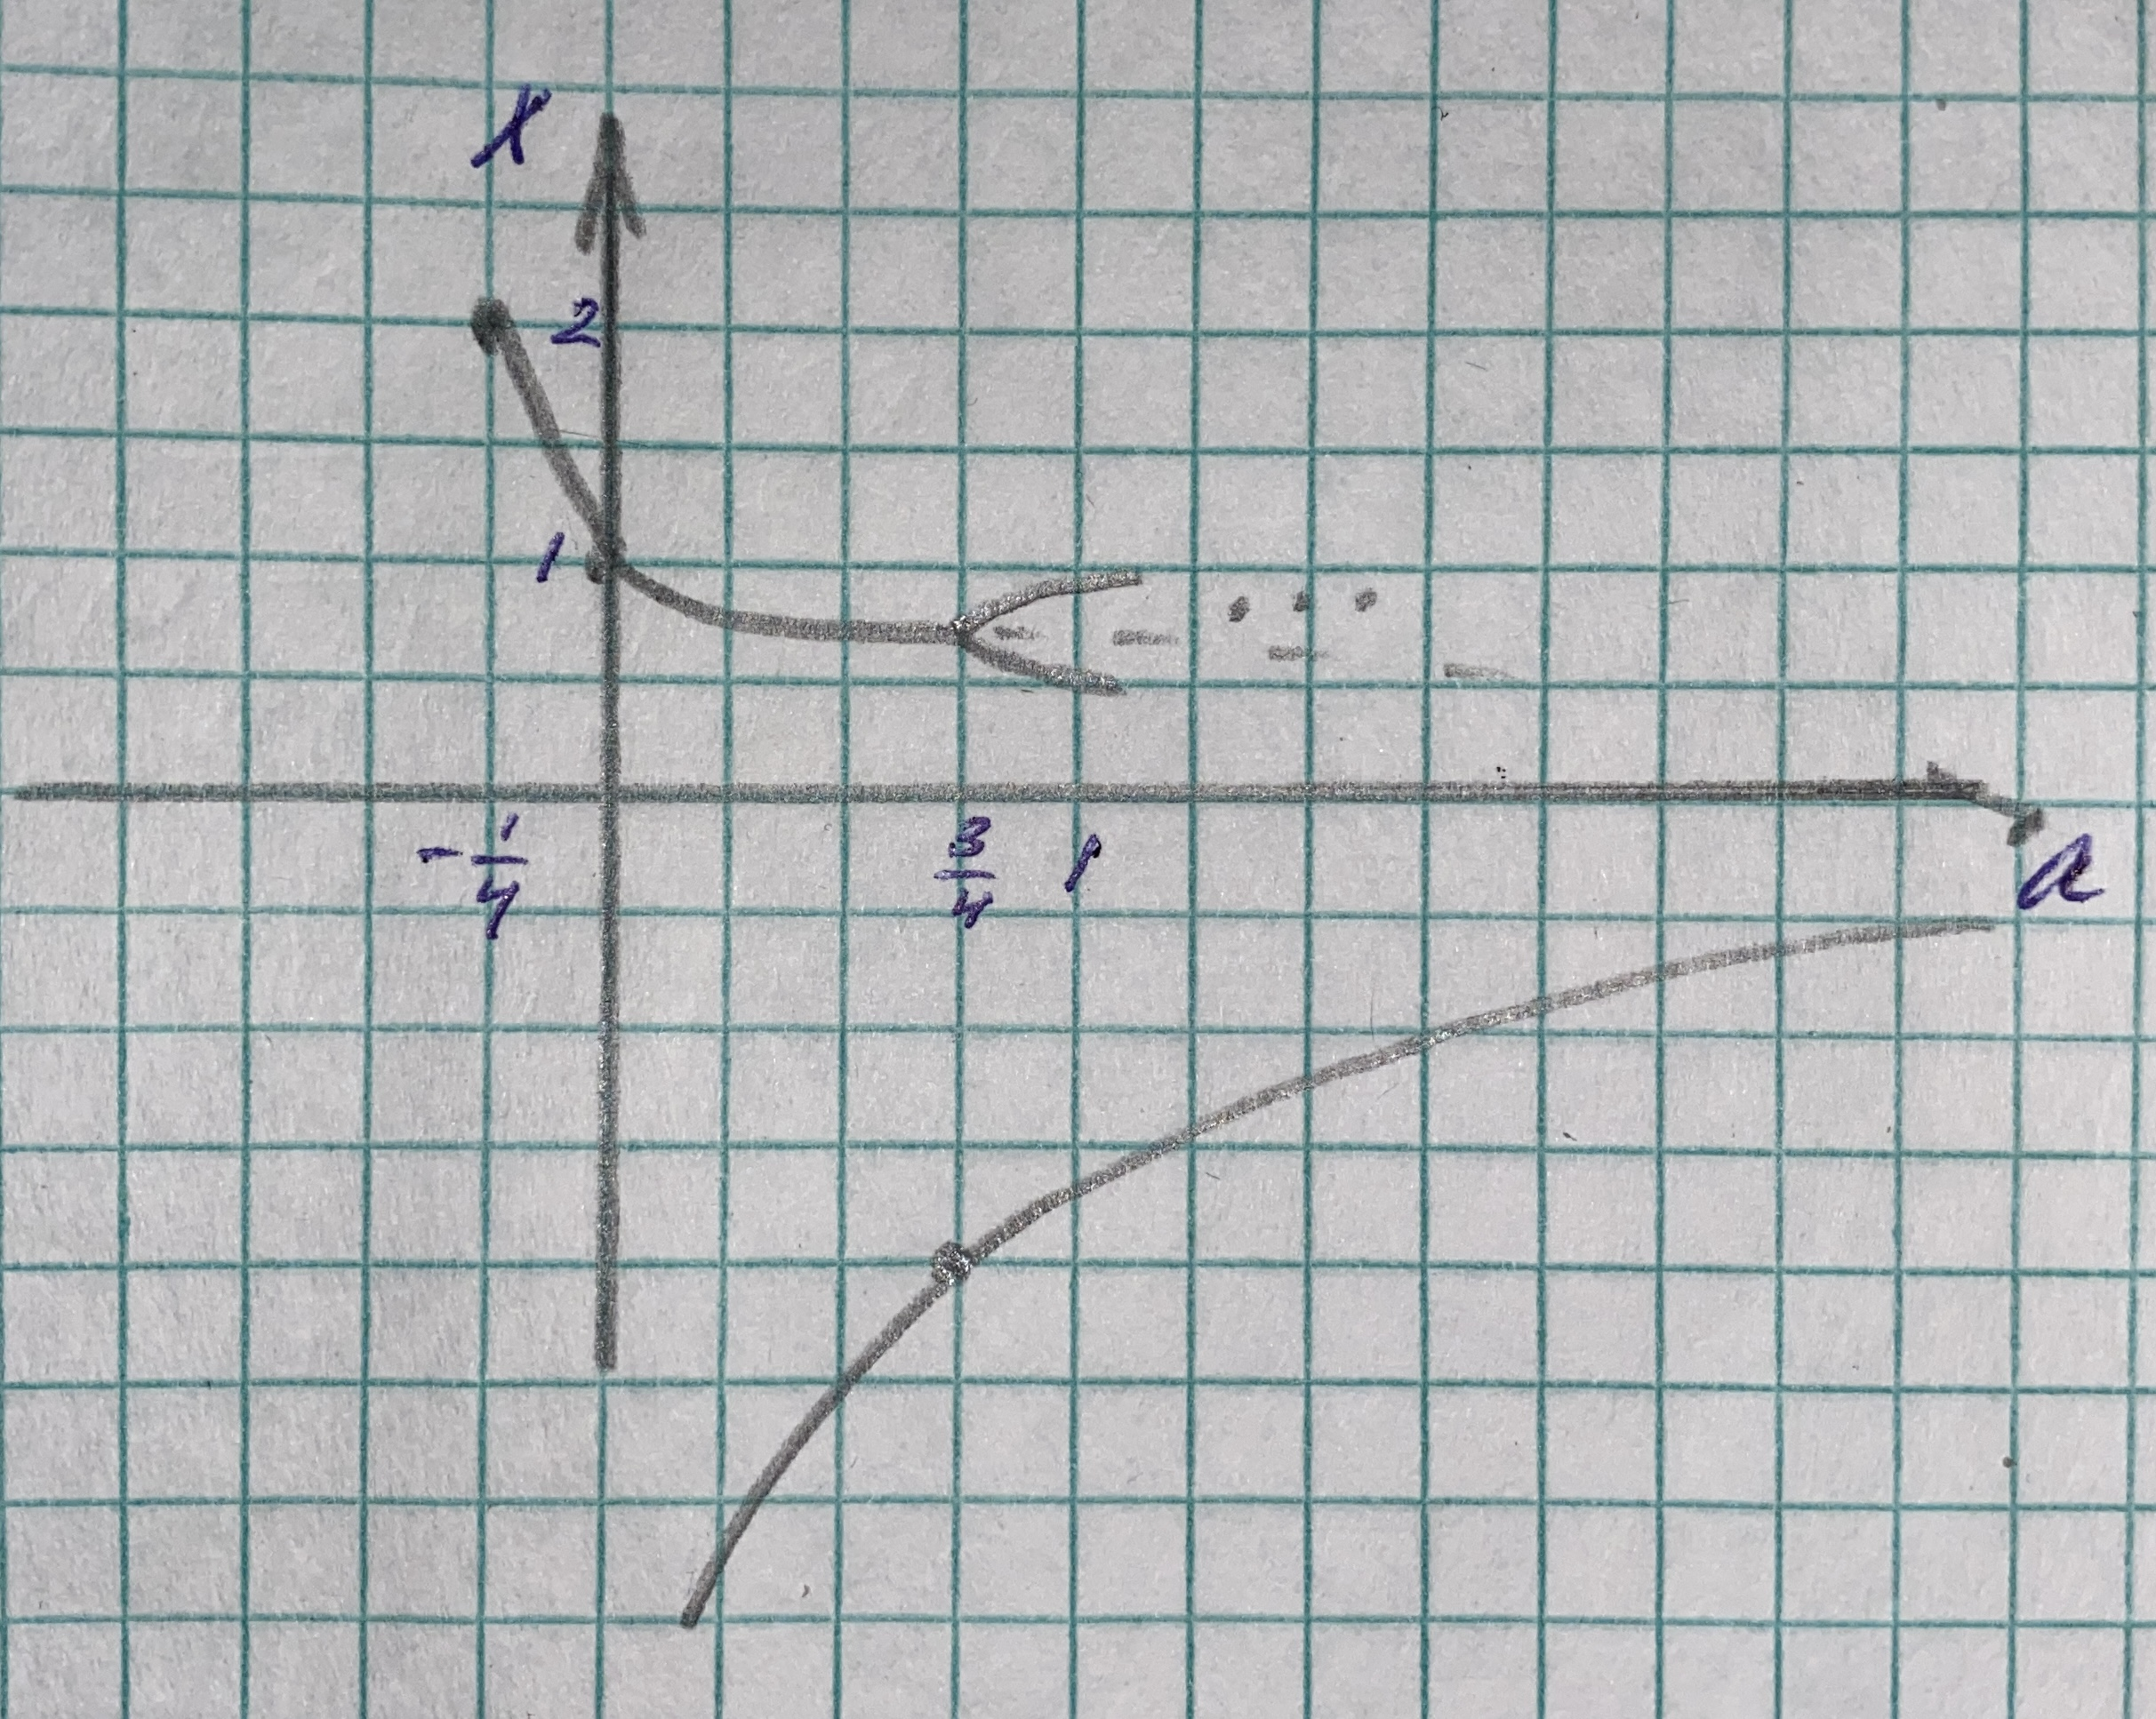
\includegraphics[scale=0.1]{feigan}}
	\caption{Часть аналитически построенного дерева Фейгенбаума}
\end{figure}
\subsection{Численно построить дерево Фейгенбаума}
\begin{figure}[H]
	\center{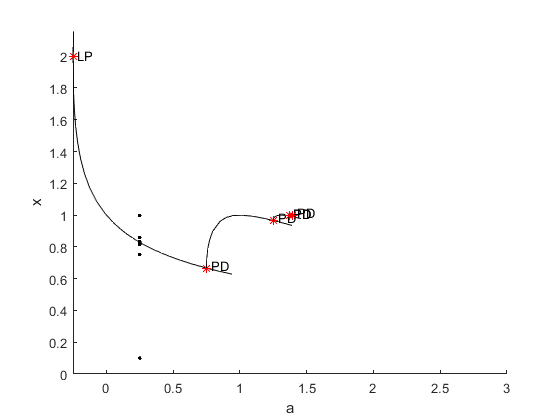
\includegraphics[scale=0.7]{1feig1}}
	\caption{Численно построенное дерево Фейгенбаума}
\end{figure}
\begin{figure}[H]
	\center{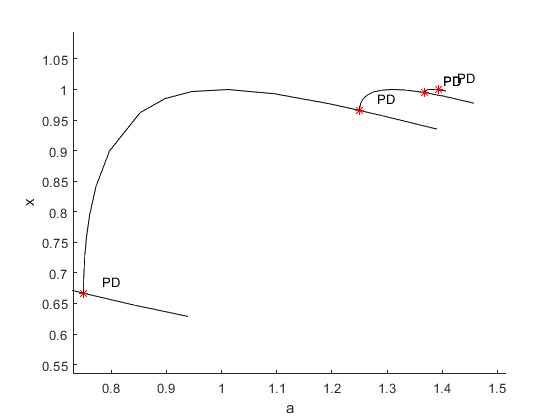
\includegraphics[scale=0.7]{1feig2}}
	\caption{Численно построенное дерево Фейгенбаума (в масштабе)}
\end{figure}

\end{document}